\documentclass{beamer}

\usepackage{tikz}
\usepackage{listings}
\usetikzlibrary{automata,positioning}
\usepackage{attrib}
\usepackage{color}
\usepackage{url}
\usepackage{todo}
\usepackage{fancyvrb}

\usetikzlibrary{er}
\title{Verifying Type Class Laws with Equational Reasoning}
\subtitle{A description by example}
\author{Lukas Hofmaier \texttt{lukas.hofmaier@hsr.ch}}
\date{June 12, 2015 \\ Progam Analysis and Transformation Seminar FS15}

\begin{document}
\maketitle
\begin{frame}
  \frametitle{Outline}
  \tableofcontents
\end{frame}

\section{Motivation}

\begin{frame}
  \frametitle{Why I'm interested in the topic?}
\begin{itemize}
\item Understanding blog post of Gabriel Gonzales
\item Understanding the advantages of purely functional programming
  \begin{itemize}
  \item Higher order functions
  \item Functional programs are often shorter
  \item {\color{red} Referential transparency makes it possible to conduct equational reasoning}
  \item It is fun
  \end{itemize}
\end{itemize}
\end{frame}

\begin{frame}[fragile]
\frametitle{What is referential transparency?}
Computation yields the same value each time it is invoked
\begin{Verbatim}[commandchars=\\\{\}]
y =  f x
g = h \textcolor{red}{y} 
\end{Verbatim}
We can replace the definition of \verb|g| with
\begin{Verbatim}[commandchars=\\\{\}]
g = h \textcolor{red}{(f x)}
\end{Verbatim}
and get the same result.

Application:
\begin{itemize}
\item Efficiency
\item Verifying correctness of a program - Equational reasoning
\end{itemize}
\end{frame}
\section{Equational Reasoning}
\subsection{Referential Transparancy}
\subsection{Reasoning about algebraic properties}

\begin{frame}
  \frametitle{What is equational reasoning?}

Equational reasoning is a method originally used in algebra.
 It's the process of proving a given property by substituting equal expressions. 
\begin{equation*}
  \label{eq:sum}
  (x+a)(x+b) = x^2 + (a+b)x+ab
\end{equation*}
\pause
\begin{equation*}
  (x+a)(x+b) = x^2 + ax + xb + ab \text{     (use distributivity)}
\end{equation*}
\pause
\begin{equation*}
x^2 + ax + xb + ab = x^2 + ax + bx + ab \text{     (use commutativity)}
\end{equation*}
\pause
\begin{equation*}
x^2 + ax + bx + ab = x^2 + (a + b)x + ab \text{     (use distributivity)}
\end{equation*}
 \footnotetext{Example taken from Graham Hutton, Programming in Haskell}
\end{frame}

\subsection{Reasoning about programs}

\begin{frame}[fragile]
  \frametitle{Reasoning about programs}
  We can reason the same way about programs.

For instance, we want to verify the following property.
\begin{verbatim}
length [x] = 1
\end{verbatim}
Given the function definition of \verb|length|.
\begin{verbatim}
length [] = 0
length (x:xs) = 1 + length xs  
\end{verbatim}

\end{frame}

\begin{frame}[fragile]
  \frametitle{Reasoning about programs}
Begin from the left-hand side \verb|length [x]| and try to get to the right-hand side \verb|1| by substituting equals-for-equals.
\begin{verbatim}
length [x]         -- [x] is the same as x:[]
\end{verbatim}
\pause
\begin{verbatim}
= length (x:[])    -- apply definition
\end{verbatim}
\pause
\begin{verbatim}
= 1 + length []    -- apply definition
\end{verbatim}
\pause
\begin{verbatim}
= 1 + 0            --  1 + 0 = 1
= 1
\end{verbatim}
\end{frame}

\subsection{Why use equational reasoning?}
\begin{frame}
\frametitle{Why use equational reasoning?}
\begin{block}{Example Property}
Correctness of a program can be specified in the form of an equation.
\begin{equation}
\text{fmap } \text{id}  =  \text{id}  
\end{equation}
We can use equational reasoning to verify if a property holds.  
\end{block}
\begin{block}{Goals of verification}
\begin{itemize}
\item Provide certainty that a program has particular properties
\item Contributes to the reliability and robustness of a software
\end{itemize}  
\end{block}
\begin{block}{Examples of use}
Example of use
\begin{itemize}
\item the first formally verified micro kernel, seL4.
\item streaming library "pipes"
\end{itemize}  
\end{block}
\end{frame}

\section{Type Classes}

\begin{frame}[fragile]
\frametitle{Type Classes}
  \begin{block}{Type classes}
    \begin{itemize}
    \item  Type class is a construct that supports overloaded functions and ad hoc polymorphism
    \item Describes the behavior of a type.
  \item An overloaded function uses different function definitions depending on the types of the arguments
  \item constrains the type variable in the type signature declaration \verb|t|. \verb|t| has to be a member of \verb|Show|.
  \end{itemize}
\end{block}
\begin{block}{Example}
\begin{Verbatim}
showlist :: Show t => [t] -> String
showlist [] = ""
showlist (x:xs) = show x ++ showlist xs
\end{Verbatim}

\end{block}
\end{frame}

\begin{frame}
\frametitle{Relation of type classes, types and values}

  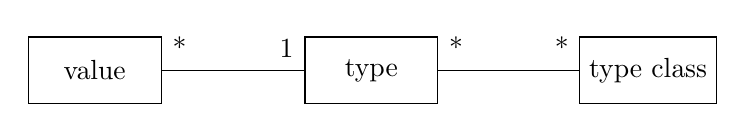
\begin{tikzpicture}[node distance=10em]
  \node[entity](type){type};
  \node[entity](typeclass)[right of=type]{type class};
  \node[entity](value)[left of=type]{value};
  \draw (type) -- (typeclass) node [very near end, above=1pt] {*} node [very near start, above=1pt] {*};
\draw (value) -- (type) node [very near end, above=1pt] {1} node [very near start, above=1pt] {*};
\end{tikzpicture}    

\end{frame}

\begin{frame}
\frametitle{Type class laws}
  \begin{itemize}
\item Type classes exhibit type class laws
\item Laws ensures expected behavior (e.g. associativity)
\item The Haskell compiler does not enforce type class laws.
\item We can use laws to apply equational reasoning
\end{itemize}  
\end{frame}

\begin{frame}
\frametitle{Relation of type classes with equational reasoning}
  \begin{figure}
  \centering
     \includegraphics[scale=0.4]{mindmap}
\end{figure}
\end{frame}

\lstset{
basicstyle=\ttfamily,
columns=fullflexible,
keepspaces=true,
captionpos=b
}

\subsection{Example Proof for a Monoid Law }

\begin{frame}[fragile]
\frametitle{Example Proof for a Monoid Law}
  Suppose we want to build a plugin system

\begin{block}{Requirements}
\begin{itemize}
\item composable
\item associative
\end{itemize}
\end{block}

\begin{block}{Usage}
\begin{verbatim}
main = do
    c <- getChar
    logto `mappend` print2stdout c
\end{verbatim}
\end{block}
\end{frame}

\begin{frame}[fragile]
\frametitle{Composability and Associativity}
\begin{block}{Composability}
\begin{Verbatim}[fontsize=\footnotesize]
composedPlugin :: Char -> IO ()
composedPlugin  = logto `mappend` print2stdout
\end{Verbatim}

\begin{Verbatim}[fontsize=\footnotesize]
-- mappend :: Plugin -> Plugin -> Plugin
\end{Verbatim}
Both arguments are of type \verb|Char -> IO ()|. The return value is also of type \verb|Char -> IO ()|.
\end{block}
\begin{block}{Associativity}
The order of evaluation must not matter.
\begin{verbatim}
composed1 = logto `mappend` (print2stdout `mappend` donothing)
composed2 = (logto `mappend` print2stdout) `mappend` donothing
\end{verbatim}
  
\end{block}
\end{frame}

\begin{frame}[fragile]
  \frametitle{Monoids to the rescue}
There is a type class for this behavior.

  \begin{itemize}
\item A monoid is when you have an associative binary function and a value which acts as an identity. Types which behave like monoids can be part of the type class \verb|Monoid|. For example list \verb|[]| under concatenation is a \verb|Monoid|.
\item The monoid laws state that \verb|mappend| must be associative.
\item If \verb|mappend| satisfies the monoid laws then we are able to add plugins without concerning about the order of evaluation.
\end{itemize}
We prove only the left identity law of the \verb|Monoid| type class.
\end{frame}

\begin{frame}
\frametitle{Example Proof for a Monoid Law}
\begin{block}{Left identity law}

    mappend mempty x = x

\end{block}
\end{frame}


\begin{frame}[fragile]
\frametitle{Associativity}
The order of evaluation must not matter.

\end{frame}


\section{Comparison of testing and proving properties}

\begin{frame}[fragile]
  \frametitle{Comparison of testing and proving properties}
  Suppose we want to check if the following equations holds
\begin{verbatim}
reverse reverse xs = xs
\end{verbatim}
How do we check that?
\begin{itemize}
\item Testing
\item Property-based testing
\item Proof that property holds
\end{itemize}

\end{frame}

\begin{frame}[fragile]
  \frametitle{Testing}
 In order to check the behavior, a function evaluates both sides of equation and compares the values
\begin{verbatim}
input = [1,2,3]
test_reverse :: Bool
test_reverse = reverse (reverse input) == input
\end{verbatim}
\end{frame}

\begin{frame}
  \frametitle{Comparison of testing and proving properties}
  \begin{description}
  \item[Testing] Code is compiled and executed. Can expose error. Cannot proof absence of errors. 
  \item[Proof] Properties hold under all circumstances.
\end{description}
\end{frame}

\begin{frame}
  \frametitle{Comparison of testing and proving properties}
\begin{figure}
  \centering
     \includegraphics[width=1\textwidth]{testing}
\end{figure}
\end{frame}

\section{Proof by structural induction}

\begin{frame}[fragile]
\frametitle{Proof by structural induction}
 \begin{description}
 \item[Base case] Prove $p(0)$ is true.
 \item[Induction step] Prove $p(n+1)$ if $p(n)$ (induction hypothesis) is true.
 \end{description}
\end{frame}

\begin{frame}[fragile]
\frametitle{Example proof by structural induction}
The length of two concatenated lists $xs$ and $ys$, is the same as the sum of the length of $xs$ and the length of $ys$
\begin{verbatim}
length (xs ++ ys) = length xs + length ys
\end{verbatim}

\end{frame}

\begin{frame}[fragile]
\frametitle{Base case}
We have to show that the property holds for the base case, the empty list \verb|[]|
\begin{verbatim}
length ([] ++ ys) = length [] + length ys
\end{verbatim}
\begin{columns}
  \begin{column}{.5\textwidth}
    \begin{block}{Left-hand side}
      \begin{verbatim}
length ([] ++ ys)
= length ys
\end{verbatim}
    \end{block}
  \end{column}
  \begin{column}{.5\textwidth}
    \begin{block}{Right-hand side}
\begin{verbatim}
length [] + length ys   
= 0 + length ys
= length ys
\end{verbatim}
    \end{block}
  \end{column}
\end{columns}
\end{frame}



\begin{frame}[fragile]
\frametitle{Induction step}
We have to show that if the equation holds for any list \verb|xs| then it also holds for \verb|x:xs|
\begin{verbatim}
pplength ([] ++ ys) = length [] + length ys
\end{verbatim}
\begin{columns}
  \begin{column}{.5\textwidth}
    \begin{block}{Left-hand side}
      \begin{verbatim}
length ((x:xs) ++ ys)      
= length (x:(xs ++ ys))    
= 1 + length (xs ++ ys)    
= 1 + length xs + length ys
\end{verbatim}
    \end{block}
  \end{column}
  \begin{column}{.5\textwidth}
    \begin{block}{Right-hand side}
\begin{verbatim}
length (x:xs) + length ys
1 + length xs + length ys
length [] + length ys   
\end{verbatim}
    \end{block}
  \end{column}
\end{columns}

\end{frame}




\begin{frame}
  \frametitle{For Further Reading}

  \begin{thebibliography}{Subramaniam, 2011}

\bibitem{hutton}
Graham Hutton,
Programming in Haskell,
Cambridge University Press,
2007.

\bibitem{gonzales}
Gabriel Gonzales,
Equational reasoning at scale, 
\url{http://www.haskellforall.com}.

\end{thebibliography}
\end{frame}

\appendix

\begin{frame}[fragile]
  \frametitle{An Applicative can be a monoid}
\begin{figure}
  \centering
     \includegraphics[width=0.7\textwidth]{monoid}
\end{figure}
\end{frame}

\begin{frame}[fragile]
  \frametitle{Proof of the monoid laws}
\begin{verbatim}
mappend mempty x                  -- apply def. mappend
= liftA2 mappend mempty x         -- apply def. mempty
= liftA2 mappend (pure mempty) x  -- apply def. of liftA2
= (pure mappend <*> pure mempty) <*> x   
 -- 3. applicative law
= pure (mappend mempty) <*> x     -- transform to lambda
= pure (\a -> mappend mempty a) <*> x   -- 1. monoid law 
= pure (\a -> a) <*> x                  -- a -> a = id
= pure id <*> x                    -- 1. applicative law
= x

\end{verbatim}

\end{frame}
\end{document}
%%% Local Variables: 
%%% mode: latex
%%% TeX-master: t
%%% End: 
